\documentclass[11pt]{article}
\usepackage[left=2cm, top=1.5cm, right=2cm, bottom=1.5cm]{geometry}
\usepackage[utf8]{inputenc}
\usepackage[T1]{fontenc}
\usepackage[french]{babel}
\usepackage{graphicx}
\usepackage{graphics}
\usepackage{amsmath}
\usepackage{tikz}
\usepackage{xcolor} 
\usepackage{mathtools}
\usepackage{parskip}
\usepackage{subcaption}
\usepackage[export]{adjustbox}
\usepackage{hyperref}

\title{\vspace{-2cm}\textbf{TP 3 - Corde vibrante}}
\author{\vspace{-0.5cm}MENARD Alexandre - VIEILLEDENT Florent}
% \setlength{\parindent}{1cm}
\date{\vspace{-0.7cm}}

\begin{document}
\maketitle

L'étude des fréquences de résonance des matériaux, en particulier celles des cordes vibrantes en acier ici, trouve des applications dans de nombreux domaines 
comme la RMN (Résonance Magnétique Nucléaire) faisant entrer en résonance les molécules à l'aide d'un champ magnétique issu d'une onde radio. Le signal de retour provenant
de la molécule permet alors d'obtenir des informations sur sa composition. 
Notre travail ici consistera alors à caractériser les cordes en vibration et leurs différents modes de vibrations. Nous identifierons les paramètres pertinents pour faire
varier le son émis par ces dernieres. Enfin, nous étudierons la complexité des sons émis selon la source de contraintes (pincements ou bobine excitatrice).

\section{Paramètres et propriétés du son émis par la corde}
\subsection{Détermination des paramètres influençant le son émis}

Dans un premier temps, on s'intéresse à déterminer quels sont les paramètres modifiant le son émis par la corde, et vérifier la conservation de la fréquence 
de vibration le long de la corde.

Pour cela, nous fixons aux deux extrémités la corde, et l'on positionne les points d'appui pour avoir la plus grande longueur possible. Nous disposons une masse de $m=250g$ sur le levier
en s'assurant qu'il soit horizontal. Nous pincons ensuite la corde et nous écoutons le son à l'oreille.

Première observation, un allongement de la corde fait baisser la fréquence du son (son de plus en plus grave). 
Seconde observation, une augmentation de la tension augmente la fréquence (son de plus en plus aigu), la tension étant dû à la masse, la distance levier-masse, et la distance
levier-(support de la corde) comme nous le verrons dans une prochaine partie, une variation d'un de ces paramètres induit donc une variation de fréquence. Pour l'instant, 
nous avons pu montré qu'une augmentation de la masse augmente la fréquence, mais nous ne pouvons pas prédire l'ordre de proportionnalité entre tension et fréquence.

Quant au signal observé par l'oscilloscope et la bobine de détection, le signal est difficilement caractérisable car il est composé d'un grand nombre de fréquences, ce que
l'on confirme à l'aide d'une transformée de Fourier.

Enfin, nous installons une bobine émettrice à un GBF  et nous comparons le signal émis par la bobine émettrice au signal reçu par la bobine réceptrice.
Nous remarquons que lorsque les deux bobines sont à une distance supérieure à environ $20cm$, le signal reçu n'est plus composé d'une seule fréquence, le son est complexe.
Cependant, il est important de noter que le signal reçu est toujours composé du signal émis (on remarque que les extremas entre signal reçu et émis sont simulanées), mais une fréquence supplémentaire
entre en compte dans le signal. 

On se place alors dans le cadre d'une distance émetteur-récepteur inférieure à $20cm$ et l'on observe un signal sinusoidal reçu de même périodicité que le signal reçu. Pour comparer les fréquences,
nous utilisons les curseurs en mesurant la fréquence maximale et minimale. On obtient alors pour la fréquence du signal émis $\nu_e = 623 \pm 10 Hz$ et pour le signal reçu $\nu_r = 629 \pm 12 Hz$. Nous pourrons alors supposer
que la fréquence est constante le long du système. On suppose que la fréquence parasite observé lorsque les capteurs sont éloignés est dû à la sensibilité du capteur trop faible et une amplitude de l'onde trop petite. 

\break

\begin{figure}[h!]
    \centering
    \begin{subfigure}{.5\textwidth}
      \centering
        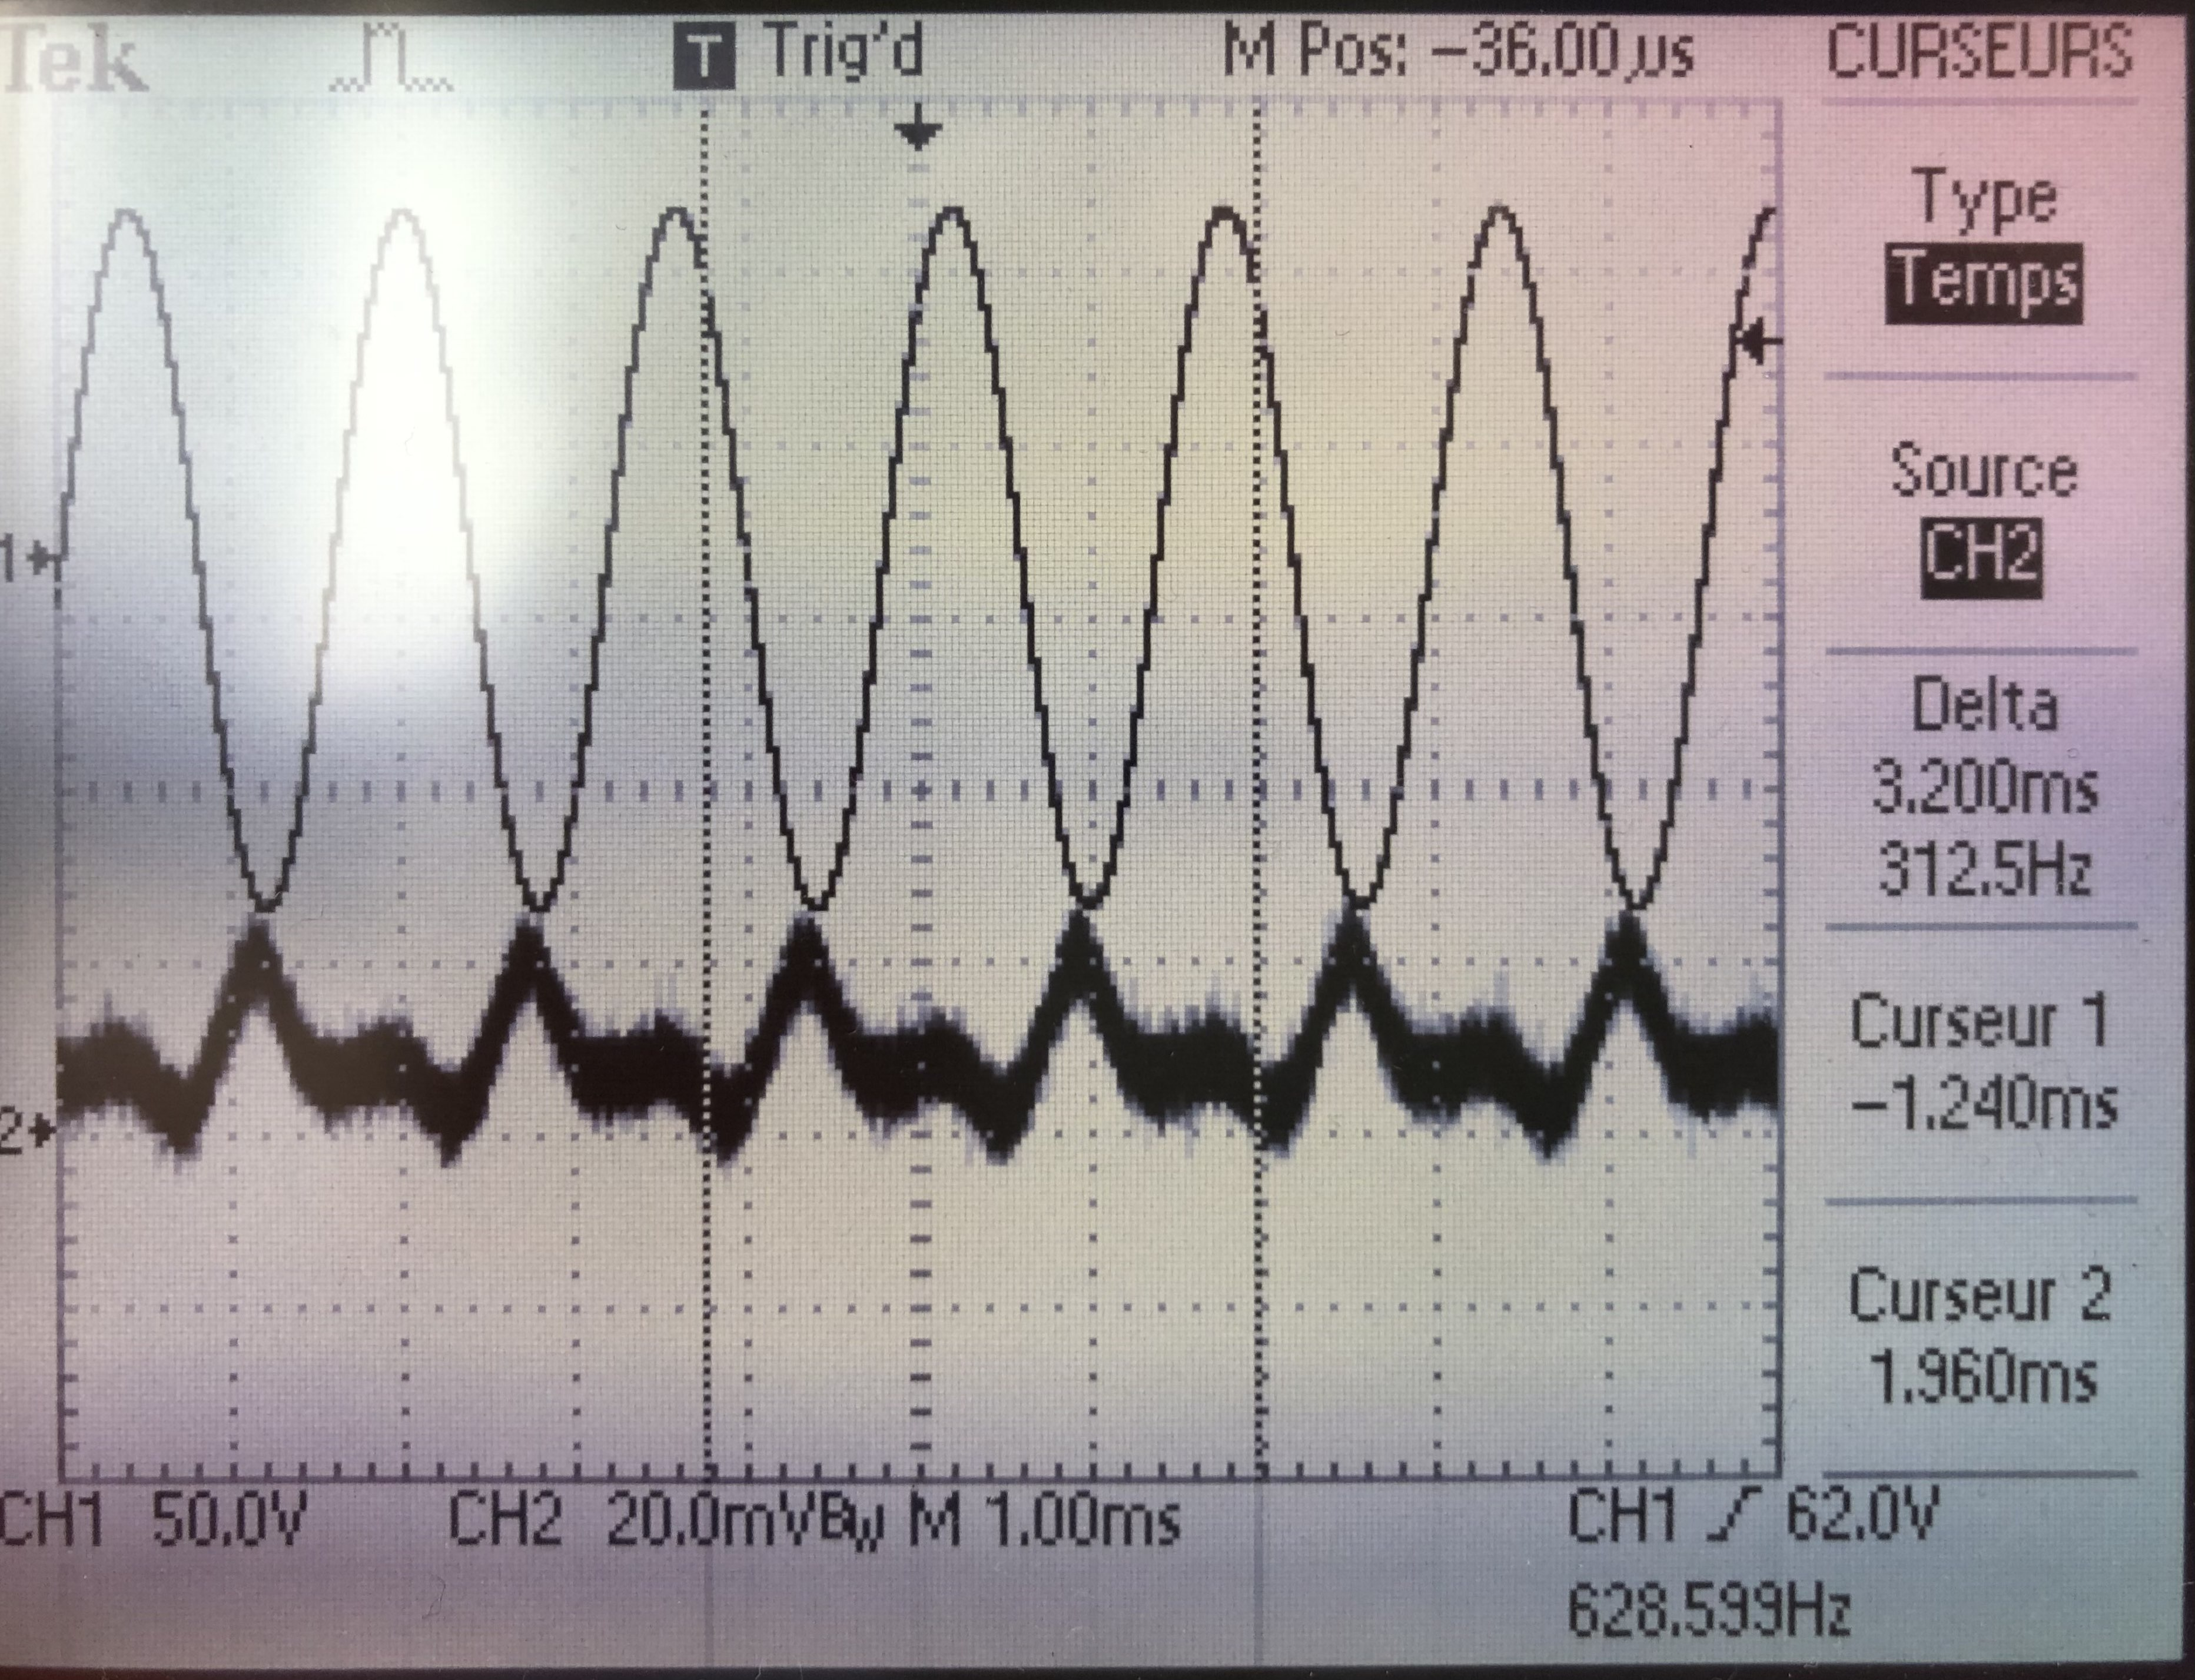
\includegraphics[width=.7\linewidth]{img/son_complexe.png}
      \caption{Distance $d>20cm$}
    \end{subfigure}%
    \begin{subfigure}{.5\textwidth}
      \centering
      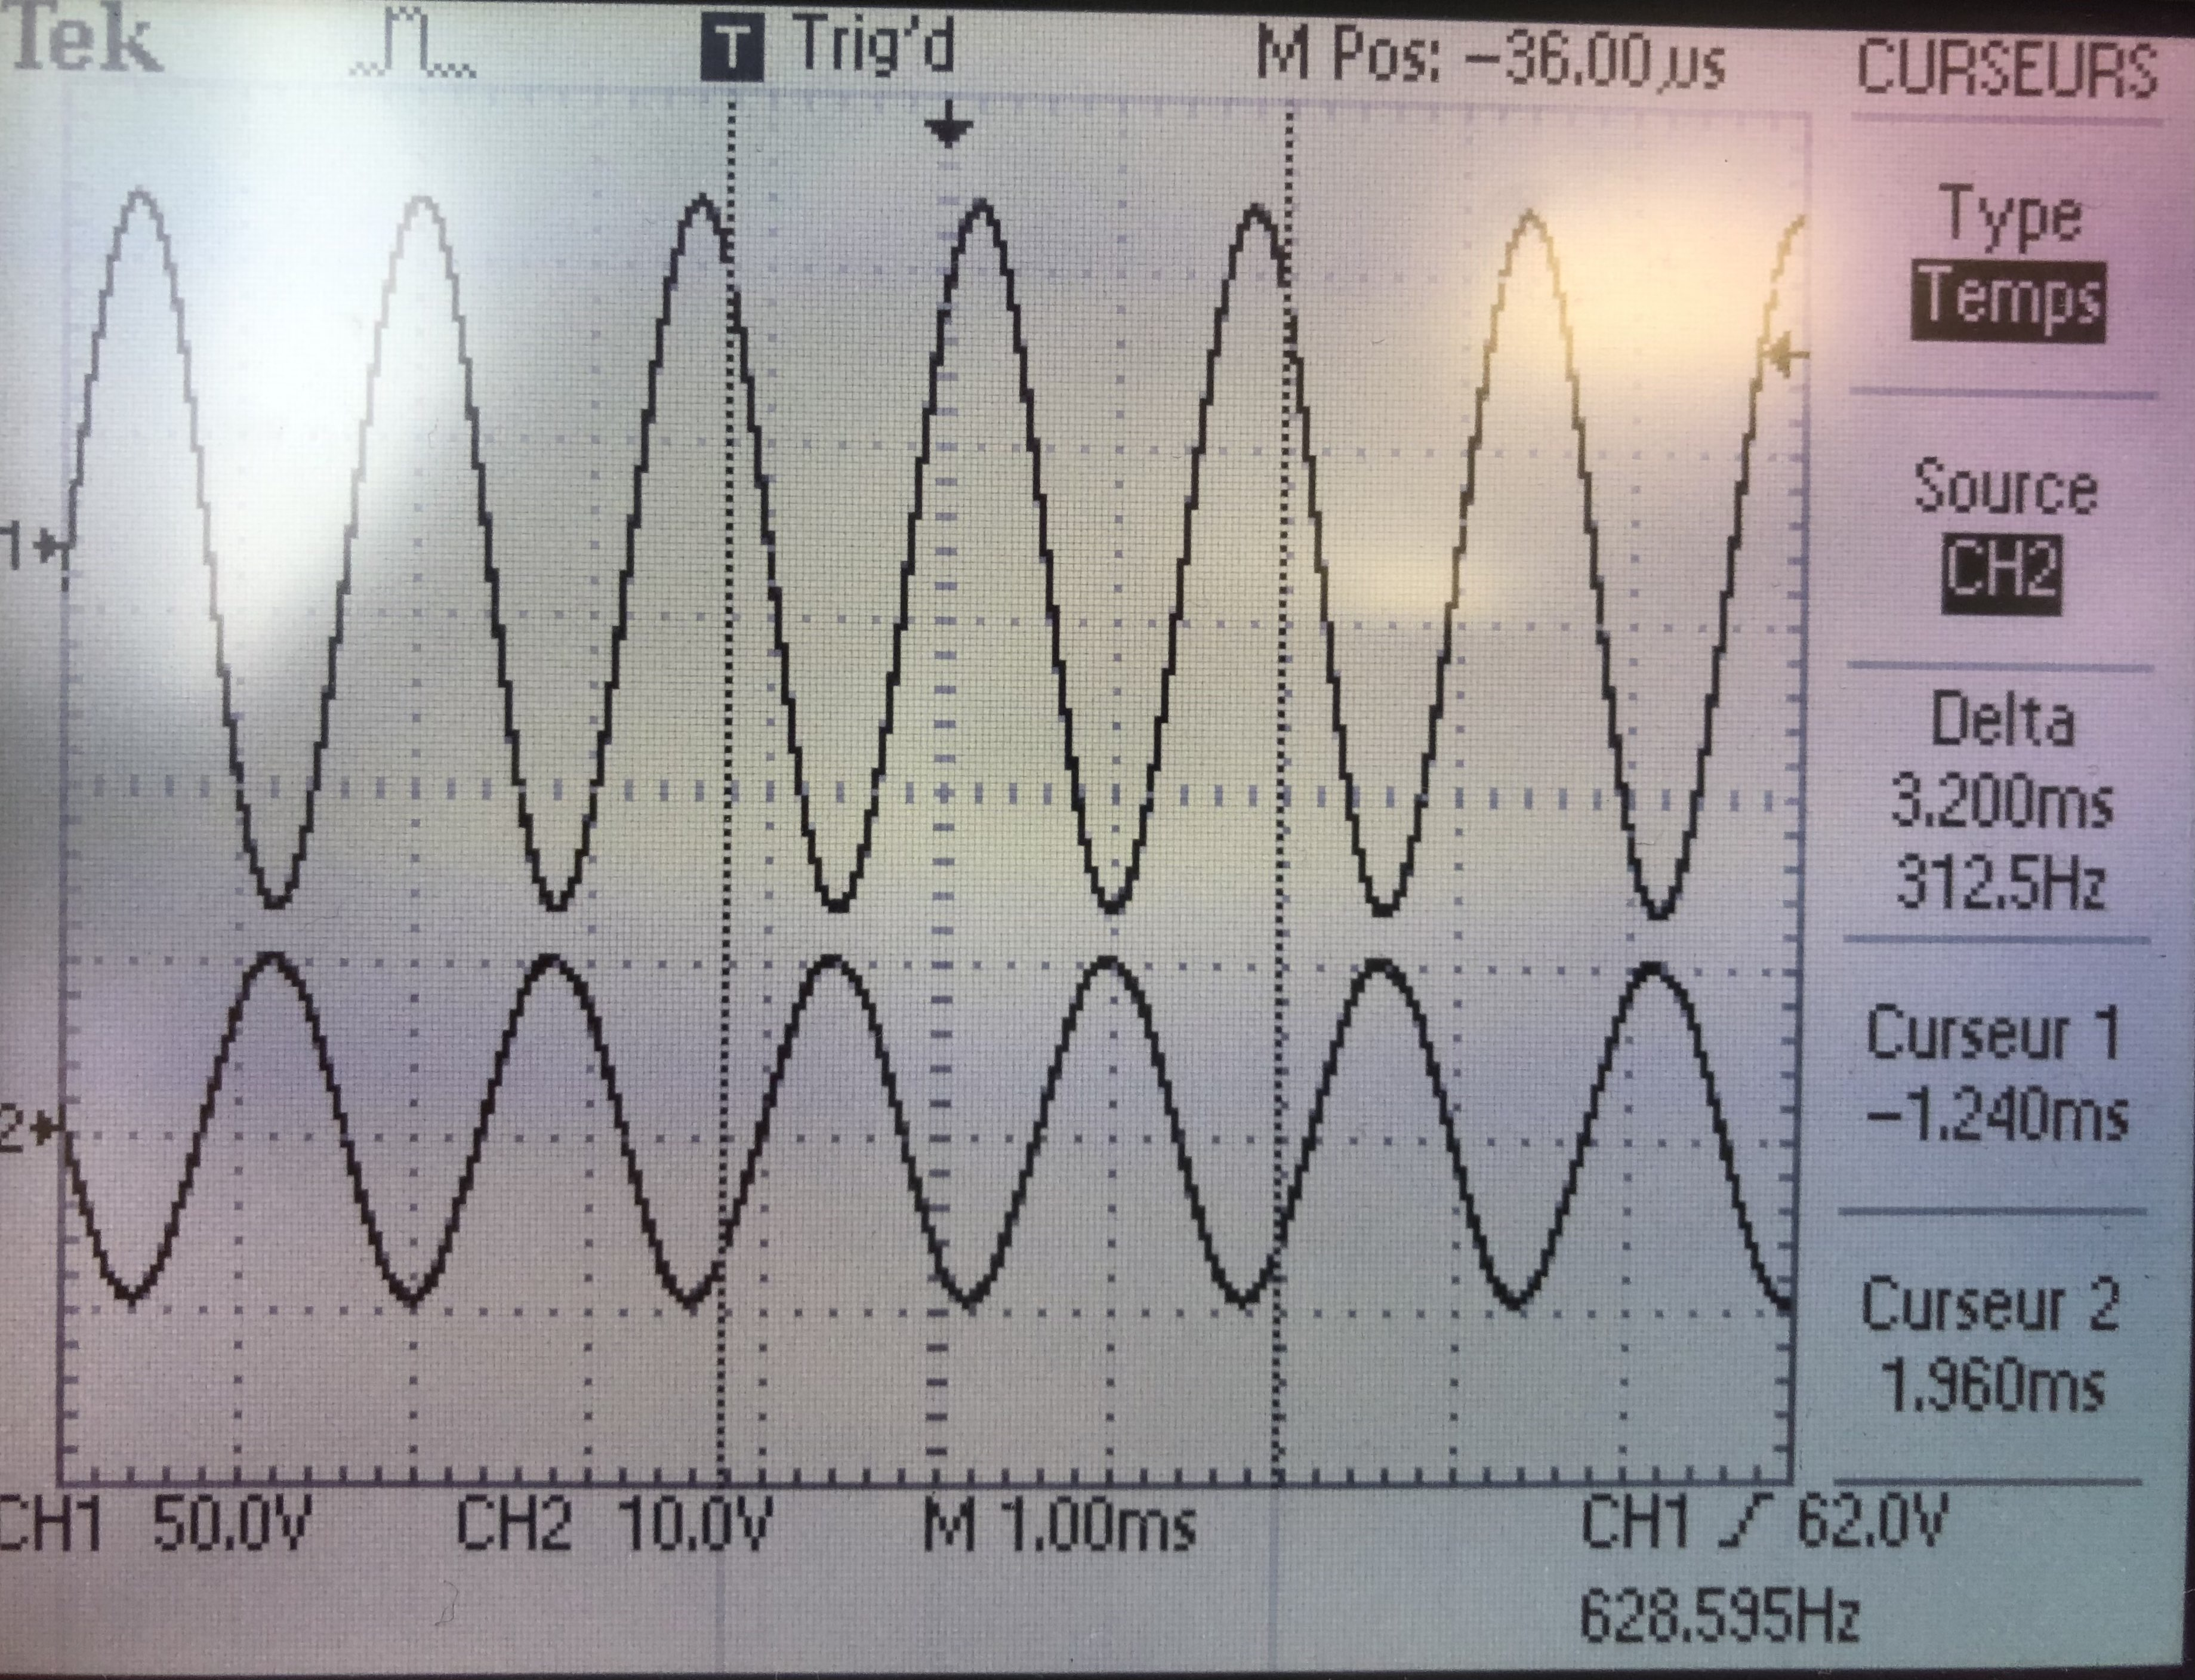
\includegraphics[width=.7\linewidth]{img/son_simple.png}
      \caption{Distance $d<20cm$}
    \end{subfigure}
    \caption*{Signal reçu et émis selon la distance émetteur-récepteur}
\end{figure}

\subsection{Propriétés de la corde}

\begin{figure}[!h]
    \begin{center}
        \resizebox{0.5\textwidth}{3cm}{
            

\tikzset{every picture/.style={line width=0.75pt}} %set default line width to 0.75pt        

\begin{tikzpicture}[x=0.75pt,y=0.75pt,yscale=-1,xscale=1]
%uncomment if require: \path (0,181); %set diagram left start at 0, and has height of 181

%Straight Lines [id:da7574645445741319] 
\draw    (40,100) -- (150,100) ;
%Shape: Circle [id:dp12384044814145212] 
\draw  [fill={rgb, 255:red, 0; green, 0; blue, 0 }  ,fill opacity=1 ] (147.5,100) .. controls (147.5,98.62) and (148.62,97.5) .. (150,97.5) .. controls (151.38,97.5) and (152.5,98.62) .. (152.5,100) .. controls (152.5,101.38) and (151.38,102.5) .. (150,102.5) .. controls (148.62,102.5) and (147.5,101.38) .. (147.5,100) -- cycle ;
%Shape: Circle [id:dp1853264368048282] 
\draw  [fill={rgb, 255:red, 0; green, 0; blue, 0 }  ,fill opacity=1 ] (37.5,100) .. controls (37.5,98.62) and (38.62,97.5) .. (40,97.5) .. controls (41.38,97.5) and (42.5,98.62) .. (42.5,100) .. controls (42.5,101.38) and (41.38,102.5) .. (40,102.5) .. controls (38.62,102.5) and (37.5,101.38) .. (37.5,100) -- cycle ;
%Shape: Circle [id:dp9952436517911716] 
\draw  [fill={rgb, 255:red, 0; green, 0; blue, 0 }  ,fill opacity=1 ] (147.5,50) .. controls (147.5,48.62) and (148.62,47.5) .. (150,47.5) .. controls (151.38,47.5) and (152.5,48.62) .. (152.5,50) .. controls (152.5,51.38) and (151.38,52.5) .. (150,52.5) .. controls (148.62,52.5) and (147.5,51.38) .. (147.5,50) -- cycle ;
%Straight Lines [id:da7613717692542328] 
\draw    (150,100) -- (150,50) ;
%Straight Lines [id:da02667716492108574] 
\draw    (40,100) -- (40,138) ;
\draw [shift={(40,140)}, rotate = 270] [color={rgb, 255:red, 0; green, 0; blue, 0 }  ][line width=0.75]    (10.93,-3.29) .. controls (6.95,-1.4) and (3.31,-0.3) .. (0,0) .. controls (3.31,0.3) and (6.95,1.4) .. (10.93,3.29)   ;
%Straight Lines [id:da20520349835399254] 
\draw    (150,50) -- (188,50) ;
\draw [shift={(190,50)}, rotate = 180] [color={rgb, 255:red, 0; green, 0; blue, 0 }  ][line width=0.75]    (10.93,-3.29) .. controls (6.95,-1.4) and (3.31,-0.3) .. (0,0) .. controls (3.31,0.3) and (6.95,1.4) .. (10.93,3.29)   ;
%Straight Lines [id:da27463252778080394] 
\draw    (150,50) -- (360,50) ;
%Shape: Circle [id:dp7429974867548343] 
\draw  [fill={rgb, 255:red, 0; green, 0; blue, 0 }  ,fill opacity=1 ] (357.5,50) .. controls (357.5,48.62) and (358.62,47.5) .. (360,47.5) .. controls (361.38,47.5) and (362.5,48.62) .. (362.5,50) .. controls (362.5,51.38) and (361.38,52.5) .. (360,52.5) .. controls (358.62,52.5) and (357.5,51.38) .. (357.5,50) -- cycle ;
%Straight Lines [id:da05926405279431912] 
\draw    (250,130) -- (250,92) ;
\draw [shift={(250,90)}, rotate = 90] [color={rgb, 255:red, 0; green, 0; blue, 0 }  ][line width=0.75]    (10.93,-3.29) .. controls (6.95,-1.4) and (3.31,-0.3) .. (0,0) .. controls (3.31,0.3) and (6.95,1.4) .. (10.93,3.29)   ;
%Straight Lines [id:da2913495095845946] 
\draw    (250,130) -- (288,130) ;
\draw [shift={(290,130)}, rotate = 180] [color={rgb, 255:red, 0; green, 0; blue, 0 }  ][line width=0.75]    (10.93,-3.29) .. controls (6.95,-1.4) and (3.31,-0.3) .. (0,0) .. controls (3.31,0.3) and (6.95,1.4) .. (10.93,3.29)   ;
%Shape: Circle [id:dp44657389872182063] 
\draw  [fill={rgb, 255:red, 0; green, 0; blue, 0 }  ,fill opacity=1 ] (210,137.5) .. controls (210,136.12) and (211.12,135) .. (212.5,135) .. controls (213.88,135) and (215,136.12) .. (215,137.5) .. controls (215,138.88) and (213.88,140) .. (212.5,140) .. controls (211.12,140) and (210,138.88) .. (210,137.5) -- cycle ;
%Shape: Circle [id:dp5978581409759287] 
\draw   (204.38,137.5) .. controls (204.38,133.01) and (208.01,129.38) .. (212.5,129.38) .. controls (216.99,129.38) and (220.63,133.01) .. (220.63,137.5) .. controls (220.63,141.99) and (216.99,145.63) .. (212.5,145.63) .. controls (208.01,145.63) and (204.38,141.99) .. (204.38,137.5) -- cycle ;

% Text Node
\draw (151,102.4) node [anchor=north west][inner sep=0.75pt]    {$O$};
% Text Node
\draw (47,116.4) node [anchor=north west][inner sep=0.75pt]    {$\vec{P}$};
% Text Node
\draw (27,82.4) node [anchor=north west][inner sep=0.75pt]    {$P$};
% Text Node
\draw (131,22.4) node [anchor=north west][inner sep=0.75pt]    {$C$};
% Text Node
\draw (161,22.4) node [anchor=north west][inner sep=0.75pt]    {$\vec{T}$};
% Text Node
\draw (231,72.4) node [anchor=north west][inner sep=0.75pt]    {$y$};
% Text Node
\draw (291,112.4) node [anchor=north west][inner sep=0.75pt]    {$x$};
% Text Node
\draw (217,140.9) node [anchor=north west][inner sep=0.75pt]    {$z$};
% Text Node
\draw (87,82.4) node [anchor=north west][inner sep=0.75pt]    {$l$};
% Text Node
\draw (137,62.4) node [anchor=north west][inner sep=0.75pt]    {$d$};


\end{tikzpicture}

        }
    \end{center}
    \caption{Schéma du montage pour l'application du théorème du moment cinétique}
    \label{fig:montage_simple}
\end{figure}

Le montage dispose de différents paramètres modifiables et non modifiables, à savoir la distance $d=OC=2.3 \pm 0.2 cm$ que l'on mesure du centre de la charnière à la corde, la distance $l=OP=9.6 \pm 0.2 \ cm$ que l'on mesure
du centre de la charnière au crochet tenant les poids. Le poids $m$ en bout de levier que l'on mesure à l'aide d'une balance. Enfin, on notera $L$ la longueur de la corde d'un point d'appui à l'autre que
l'on mesure à l'aide de la règle présente sur le sonomètre.

Le système étant à l'équilibre, on a directement:
\begin{align*}
    \frac{d \vec{L_0}}{dt} = \vec{0} & \Rightarrow \vec{OC} \wedge \vec{T} + \vec{OP} \wedge \vec{P} = \vec{0} \\
    & \Rightarrow dT = mlg \\
    & \Rightarrow T = \frac{mlg}{d}
\end{align*}

Il est important de noter que le levier porte-masse doit être à l'horizontal car dans le cas contraire, pour compenser le moment du poids, la tension ne sera plus
uniquement selon l'axe de la corde, or c'est exactement l'hypothèse de la résolution de l'équation de propagation des ondes. 

\break
\section{Oscillations libres et forcées}
\subsection{Théorie}
\begin{figure}[!h]
    \begin{center}
        \resizebox{0.8\textwidth}{3.2cm}{
            

\tikzset{every picture/.style={line width=0.75pt}} %set default line width to 0.75pt        

\begin{tikzpicture}[x=0.75pt,y=0.75pt,yscale=-1,xscale=1]
%uncomment if require: \path (0,300); %set diagram left start at 0, and has height of 300

%Straight Lines [id:da0009012527440910301] 
\draw  [dash pattern={on 0.84pt off 2.51pt}]  (40,80) -- (140,80) ;
\draw [shift={(140,80)}, rotate = 180] [color={rgb, 255:red, 0; green, 0; blue, 0 }  ][line width=0.75]    (0,5.59) -- (0,-5.59)   ;
\draw [shift={(40,80)}, rotate = 180] [color={rgb, 255:red, 0; green, 0; blue, 0 }  ][line width=0.75]    (0,5.59) -- (0,-5.59)   ;
%Shape: Wave [id:dp3427801797334673] 
\draw   (40,80) .. controls (56.31,95.37) and (71.9,110) .. (90,110) .. controls (108.1,110) and (123.69,95.37) .. (140,80) ;
%Straight Lines [id:da24216177439384023] 
\draw  [dash pattern={on 0.84pt off 2.51pt}]  (190,80) -- (290,80) ;
\draw [shift={(290,80)}, rotate = 180] [color={rgb, 255:red, 0; green, 0; blue, 0 }  ][line width=0.75]    (0,5.59) -- (0,-5.59)   ;
\draw [shift={(190,80)}, rotate = 180] [color={rgb, 255:red, 0; green, 0; blue, 0 }  ][line width=0.75]    (0,5.59) -- (0,-5.59)   ;
%Shape: Wave [id:dp585912418227907] 
\draw   (190,80) .. controls (198.07,95.37) and (205.79,110) .. (214.75,110) .. controls (223.71,110) and (231.43,95.37) .. (239.5,80) .. controls (247.57,64.63) and (255.29,50) .. (264.25,50) .. controls (273.21,50) and (280.93,64.63) .. (289,80) .. controls (289.33,80.64) and (289.67,81.27) .. (290,81.9) ;
%Straight Lines [id:da6702335390443264] 
\draw  [dash pattern={on 0.84pt off 2.51pt}]  (340,80) -- (440,80) ;
\draw [shift={(440,80)}, rotate = 180] [color={rgb, 255:red, 0; green, 0; blue, 0 }  ][line width=0.75]    (0,5.59) -- (0,-5.59)   ;
\draw [shift={(340,80)}, rotate = 180] [color={rgb, 255:red, 0; green, 0; blue, 0 }  ][line width=0.75]    (0,5.59) -- (0,-5.59)   ;
%Shape: Wave [id:dp21235427553707686] 
\draw   (340,80) .. controls (345.46,95.37) and (350.69,110) .. (356.75,110) .. controls (362.81,110) and (368.04,95.37) .. (373.5,80) .. controls (378.96,64.63) and (384.19,50) .. (390.25,50) .. controls (396.31,50) and (401.54,64.63) .. (407,80) .. controls (412.46,95.37) and (417.69,110) .. (423.75,110) .. controls (429.63,110) and (434.72,96.25) .. (440,81.41) ;
%Shape: Wave [id:dp4594230734819942] 
\draw   (140,80) .. controls (123.69,64.63) and (108.1,50) .. (90,50) .. controls (71.9,50) and (56.31,64.63) .. (40,80) ;
%Shape: Wave [id:dp2703843813543716] 
\draw   (289.98,79.96) .. controls (281.92,95.33) and (274.21,109.96) .. (265.25,109.96) .. controls (256.29,109.97) and (248.56,95.34) .. (240.48,79.99) .. controls (232.4,64.63) and (224.68,50.01) .. (215.72,50.01) .. controls (206.76,50.02) and (199.05,64.65) .. (190.98,80.01) .. controls (190.65,80.65) and (190.32,81.28) .. (189.99,81.91) ;
%Shape: Wave [id:dp6864186800918131] 
\draw   (340,80) .. controls (345.46,64.63) and (350.69,50) .. (356.75,50) .. controls (362.81,50) and (368.04,64.63) .. (373.5,80) .. controls (378.96,95.37) and (384.19,110) .. (390.25,110) .. controls (396.31,110) and (401.54,95.37) .. (407,80) .. controls (412.46,64.63) and (417.69,50) .. (423.75,50) .. controls (429.63,50) and (434.72,63.75) .. (440,78.59) ;

% Text Node
\draw (68,132.4) node [anchor=north west][inner sep=0.75pt]    {$n=1$};
% Text Node
\draw (218,132.4) node [anchor=north west][inner sep=0.75pt]    {$n=2$};
% Text Node
\draw (368,132.4) node [anchor=north west][inner sep=0.75pt]    {$n=3$};


\end{tikzpicture}

        }
    \end{center}
    \caption{Allure de la corde du mode fondamentale à la seconde harmonique ($n=3$)}
    \label{fig:mode_fonda}
\end{figure}

Notons $L$ la longueur de la corde, on remarque grâce aux conditions aux limites qu'il existe une relation entre $L$ et la longueur d'onde $\lambda$.
\begin{equation}
    2L = n\lambda \Rightarrow \nu_n = \frac{nc}{2L} = \nu_n = \frac{n}{2L}\sqrt{\frac{T}{\mu}}
\end{equation}

Pour une masse de $m=350 \pm 0.1g$ et une longueur de corde de $L=60 \pm 0.2cm$, on s'attend alors à une fréquence fondamentale $\nu_f = 90 \pm 5 Hz$.

\subsection{Oscillations libres}
Dans cette expérience, nous allons pincer la corde et mesurer par transformée de fourier les écarts entre deux pics de fréquence ayant une haute amplitude.
En pincant la corde, nous observons un ventre au centre de la corde, avec une forme proche d'un mode fondamentale. Cependant, en effectuant une FFT sur le signal reçu,
nous sommes dans l'incapacité d'observer des pics distincts, le signal est composé d'une multitude de fréquences.

Pour s'affranchir du problème, nous allons générer une contrainte sur la corde à l'aide du GBF en positionnant la fréquence émise à $\nu_e = 583.9 Hz$ et on observe
les pics de fréquence obtenus. A l'aide des curseurs, nous mesurons l'écart maximal et minimal entre deux pics successifs et l'on effectue la moyenne. On obtient alors:

\begin{table}[h!]
	\centering
	\begin{tabular}{||c c c c c||} 
		\hline
		Pics & 1-2 & 2-3 & 3-4 & 4-5 \\
		\hline
        $\Delta \nu$ en Hz & $580 \pm 40$ & $606 \pm 40$ & $574 \pm 40$ & $580 \pm 40$ \\
		\hline
	\end{tabular}
	\caption{Ecarts de fréquence entre deux pics successifs}
	\label{table:1}
\end{table}

Nous remarquons bien que la fréquence $\nu_e$ imposée est comprise dans les différences de fréquence entre deux pics successifs, ce qui est en accord avec la théorie qui prédit 
un écart constant entre deux harmoniques.

\break
\subsection{Oscillations forcées}
Prenons le montage avec $m=350 \pm 0.1 \ g$ et $L=40 \pm 0.2 \ cm$. Nous allons faire vibrer la corde avec le GBF et relever les fréquences où la vibration montre une amplitude
maximale, et on notera les noeuds et ventres de vibration.

Seul la masse volumique de la corde nous est donnée, on mesure avec une règle électronique le rayon de la corde $r=0.25 \pm  0.05 \ mm$ pour pouvoir calculer la section $S$ de la corde. On a la relation $\mu= S \times \rho$ avec $\rho = 7.8 \times 10^3 \ kg.m^{-3}$.
On note que cette n'est pas très précise, il faudrait calculer la masse linéique de la corden, mais il faut pour cela peser la corde ce qui n'était pas possible pendant la manipulation.

Nous partons d'une fréquence nulle et l'on augmente progressivement en sachant que la fréquence théorique fondamentale est de $\nu_f = 114 \pm 6 Hz$.
Nous observons un premier état de forte vibration avec un seul ventre au centre semblable à un mode fondamental à $\nu_1 = 27.3 \pm 3 Hz$ puis un second état 
de vibration avec un noeud central et 2 ventres à $\nu_2 = 55 \pm 3 Hz$ puis un troisième à $\nu_3 = 106.2 \pm 5Hz$ avec un noeud central et 2 ventres, ce qui est équivalent à la vibration
précédent. Nous retrouvons la fréquence prédite par la théorie cependant la fréquence initiale est divisée par 4. Jusque là, nous ne sommes pas en mesure de proposer une explication
satisfaisante à cette anomalie.

Nous répétons l'opération pour différentes longueurs $L$ et l'on obtient alors:

\begin{table}[h!]
	\centering
	\begin{tabular}{||c c c c c c c c||} 
		\hline
		$L \pm 1$ en cm & 60 & 50 & 40 & 30 & 20 & 15 & 10 \\
		\hline
        $f_{0exp}$ en Hz & $70 \pm 7$ & $84.9 \pm 7$ & $106.2 \pm 7$ & $140 \pm 7$ & $205 \pm 10$ & $295 \pm 10$ & $426 \pm 10$ \\
        $f_{0th}$ en Hz & $76 \pm 4$ & $91 \pm 5$ & $114 \pm 6$ & $152 \pm 8$ & $228 \pm 12$ & $304 \pm 16$ & $457 \pm 25$ \\
		\hline
	\end{tabular}
	\caption{Fréquence de résonance pour différentes longueurs de corde $L$}
	\label{table:2}
\end{table}

\textbf{Remarque:} Il est important de retenir que nous observons le même problème que dans l'expérience précédente, pour chaque longueur on observe un effet de résonance sur la corde
pour des fréquences $f_0/4$ et $f_0 / 2$. Les fréquences dans le tableau ne sont donc pas les fréquences fondamentales.

On trace $f_0$ en fonction de $1/L$ (figure (\ref{img:Courbe_derniere_expérience})). 
La valeur expérimental pour la pente de la droite $a_{exp}=43 \pm 2 \ Hz.m$ est en accord avec la pente théorique $a_{th}=40 \pm 10 \ Hz.m$.

Nous retrouvons bien des modes propres à la fréquence prédite $f_{0th}$ par la théorie, cependant, $f_{0th}$ est un multiple d'une fréquence fondamentale plus basse avec $\nu_{th} = 4 \nu_{f,exp}$.
On remarque que l'erreur est présente sur l'ensemble des groupes de travail, et qu'elle se propage sur chaque expérience, l'erreur est donc systématique. Cependant, les valeurs expérimentales restent prochent
de la théorie. Les observations doivent donc avoir un sens physique.
Malheureusement, nous ne sommes pas en capacité de produire une explication satisfaisante à un tel écart à la théorie, l'écart ne pouvant pas être attribué à des incertitudes. Il semble très peu probable
que l'erreur soit dû au protocole car l'erreur n'était pas présente sur les groupes précédents, en admettant que le problème aurait été soulevé par les anciens étudiants si l'erreur avait lieu.

En conclusion, nous avons montré que le son émis dépendait de la tension de la corde et de sa longueur expérimentalement (elle dépend aussi de sa masse linéique). Nous avons prouvé la conservation de la fréquence dans le système.
Enfin, nous avons réussi à observer les différents modes propres de vibration que la théorie prédit avec les ventres et noeuds de vibration. Cependant, nous sommes arrivés à des résultats en désaccord avec la théorie
sans pouvoir fournir d'explications bien que les valeurs semblent suivent une logique avec des fréquences de résonance qui ne sont que des multiples paires d'une sous-fréquence à celle prédite par la théorie. 
Pour améliorer notre protocole on peut commencer par utiliser une corde dont on connait la masse linéique pour améliorer nos calculs. 
On peut répéter notre protocole avec différents émetteurs et cordes pour voir si l'observation de sous-fréquence est reproductible.

\newpage

\section*{Annexes}

\begin{figure}[h!]
    \begin{center}
        \includegraphics*[angle=90,scale=0.4]{img/Courbes_TP3_ondes}
        \caption{Courbe de $f_0$ en fonction de $1/L$. Les incertitudes sur $1/L$ sont trop petites pour être visibles}
        \label{img:Courbe_derniere_expérience}
    \end{center}
\end{figure}

On calcule la pente et son incertitude avec la méthode des pentes extrêmes (on néglige les incertides sur L, celles ci étant faibles devant celles sur $\nu$). 
\begin{align*}
    a_{max} &=\frac{426+10-(70-7)}{10-1.7} & a_{min} &=\frac{426-10-(70+7)}{10-1.7} \\
    a_{max} &=44.9 \ Hz.m & a_{min} &= 40.8 \ Hz.m
\end{align*}

\begin{align*}
    a&=\frac{a_{max} + a_{min}}{2} &\delta a &= \frac{a_{max} - a_{min}}{2} \\
    a&=\frac{44.9 + 40.8}{2} &\delta a &= \frac{44.9 - 40.8}{2} \\
    a&= 42.9 \ Hz.m &\delta a &= 2.0 \ Hz.m
\end{align*}

On a donc $a=43 \pm 2 \ Hz.m$. On note tout de fois que notre droite ne passe pas par toutes les incertitudes, on a sûrement sous estimé les incertitudes sur $f_0$.

\newpage
On calcule la valeur théorique:

\begin{align*}
    a_{th} &= \frac{1}{2} \sqrt{\frac{T}{\mu}}\\
    a_{th}&=\frac{1}{2} \sqrt{\frac{m \times g \times l}{d \times \rho \times S}} \\
    a_{th}&=\frac{1}{2} \sqrt{\frac{0.250 \times 9.6 \times 9.81}{2.3 \times 7.8 \times 10^{3} \times \pi (0.25 \times 10^{-3})^2}} \\
    a_{th}&= 40.8 \ Hz.m
\end{align*}

On calcule l'incertitude associée:
\begin{align*}
    \delta a_{th} &= a_{th} \times [\frac{\delta r}{r}+\frac{1}{2}\left(\frac{\delta l}{l}+ \frac{\delta d}{d}\right)] \\
    \delta a_{th} &= 40.8 \times [0.2 + \frac{1}{2}\left(0.021+0.087\right)] \\
    \delta a_{th} &= 10 Hz.m
\end{align*}

On a donc $a_{th}=40\pm 10 \ Hz.m$. L'incertitude relative est importante car le mesure sur $r$ est peu précise. 

\end{document}